\section{Further Experimental Results}\label{sec:more-experiments}

\subsection{The Block Production Rate}

As expected, the confirmation latency of PoEM behaves convexly as the block production rate $g$ is varied.
This is illustrated in Figure~\ref{fig:g_latency} for fixed values of $\beta$ and $\gamma$.
The simulation methodology is the same as in Section~\ref{sec:experiment}.
For small block production rates, close to zero, we get high latency because blocks are produced very slowly.
For large block production rates, we get high latency because honest blocks effect many forks, whereas the adversarial blocks
are all chained in series, and a large confirmation parameter $k$ is required for safety.
We get optimal latency somewhere in the middle.

\begin{figure}[pt]
  \centering
  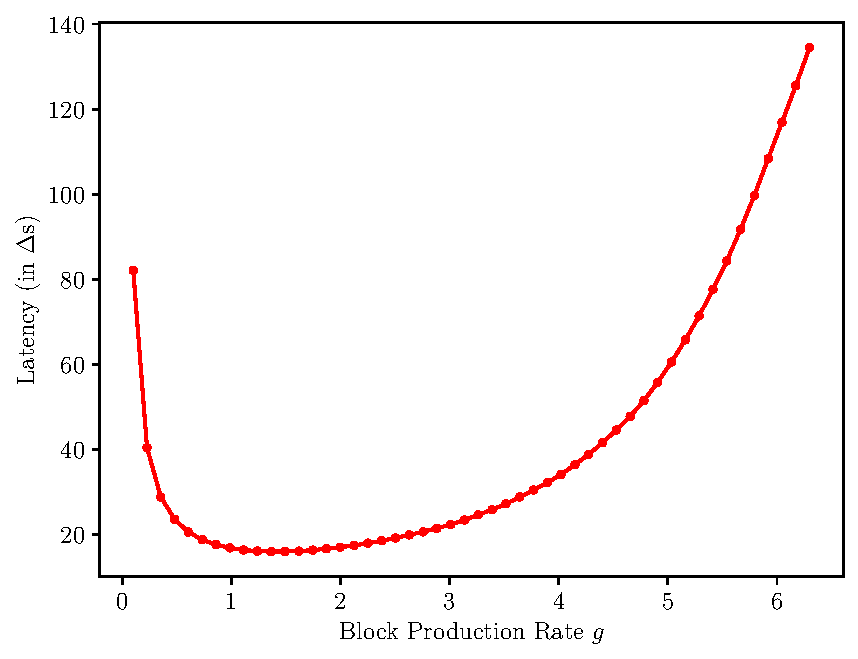
\includegraphics[width = 0.8\textwidth]{figures/g_latency.pdf}

  \caption{Fixing $\beta=0.2$ and $\gamma=0$, we plot the latency of PoEM parameterized under different block production rates $g$.
           The results were obtained by running $100{,}000$ Monte Carlo iterations per point.}
  \label{fig:g_latency}
\end{figure}

\subsection{The Bias Parameter}

In our analysis, we assumed $\gamma = 0$ for simplicity, but the $\gamma$ parameter
seems to be a promising knob to tune the performance of PoEM. While we leave
the
analytic treatment of the optimal $\gamma$ for future work, we note here that,
for given values of $g$ and $\beta$, the delay of the system behaves as illustrated
in Figure~\ref{fig:gamma_latency} for varying values of $\gamma$. This is convex, and for $\gamma \to \infty$,
the delay asymptotically approaches a value smaller than Bitcoin's. Indeed, if $\gamma$ is made sufficiently large, the bias
parameter dominates against the $-\lg\frac{H(B)}{T}$ term, and the system behaves
as if each block counts the same. However, even with $\gamma \to \infty$, PoEM provides a tie-breaker
which helps with latency. In this regime, this tie-breaker is as good as any.

\begin{figure}[h]
    \centering
    \begin{subfigure}{0.8\textwidth}
    \centering
    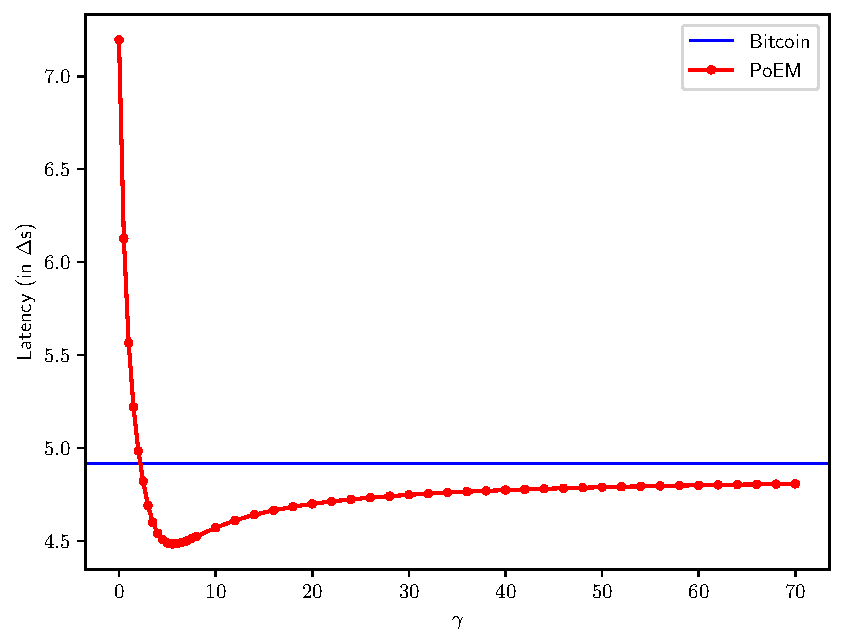
\includegraphics[width = \textwidth]{figures/gamma_latency_0.1.pdf}
    \caption{$\beta = 0.1$ and $g = 0.7$}
    \label{fig:gamma_latency_0.1}
    \end{subfigure}
    \begin{subfigure}{0.8\textwidth}
    \centering
    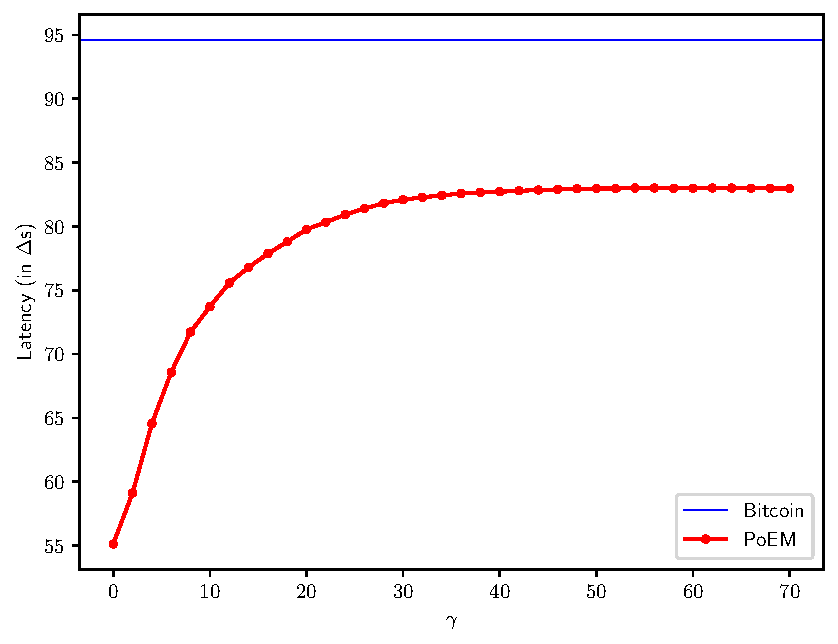
\includegraphics[width = \textwidth]{figures/gamma_latency_0.3.pdf}
    \caption{$\beta = 0.3$ and $g = 0.7$}
    \label{fig:gamma_latency_0.3}
    \end{subfigure}

  \caption{Fixing $\beta$ and $g$, we compare Bitcoin's latency against PoEM's parameterized under different $\gamma$ values
           (denser around the points of interest).
          We observe the plot is convex and for large $\gamma$, the latency
          approaches a value lower than Bitcoin's. The results were obtained by running $100{,}000$ simulations per point.}
    \label{fig:gamma_latency}
\end{figure}